\documentclass{article}

\usepackage[utf8]{inputenc}
\usepackage[ngerman]{babel}
\usepackage{amssymb}
\usepackage{amsmath}
\usepackage{graphics}
\usepackage{stmaryrd}
% Pseudocode
\usepackage{algorithm}
\usepackage[noend]{algpseudocode}
\usepackage{graphicx}
\usepackage{pdfpages}
\graphicspath{ {./images/} }

\setlength{\parindent}{0in}

\newcommand{\uebungsGruppe}{110}
\newcommand{\zettelNummer}{5}
\newcommand{\studierenderEins}{Eli Kogan-Wang (7251030)}
\newcommand{\studierenderZwei}{David Noah Stamm (7249709)}
\newcommand{\studierenderDrei}{Daniel Heins (7213874)}
\newcommand{\studierenderVier}{Tim Wolf (7269381)}

\newcounter{AufgabenCounter}
\setcounter{AufgabenCounter}{1}
\newcounter{TeilaufgabenCounter}
\newenvironment{aufgabe}{\section*{Aufgabe \theAufgabenCounter}\setcounter{TeilaufgabenCounter}{1}}{\stepcounter{AufgabenCounter}}
\newenvironment{teilaufgabe}{\paragraph*{\alph{TeilaufgabenCounter})}}{\stepcounter{TeilaufgabenCounter}}

\renewcommand{\to}{\textnormal{ to }}
\newcommand{\bigO}{\mathcal{O}}

\newcommand{\qed}{\hfill$\square$}

\begin{document}

\title{Datenstrukturen und Algorithmen \\ Heimübung \zettelNummer{}}
\author{\studierenderEins{} \\
  \studierenderZwei{} \\
  \studierenderDrei{} \\
  \studierenderVier{}}

\maketitle

% Aufgabe 1
\begin{aufgabe}
  % Angenommen, die Funktion Partiton teilt Teilarrays der Größen n immer in zwei Teilarrays auf,
  % von denen eines (1 − α) · n Elemente und das andere α · n Elemente enthält, mit 1
  % 2 ≤ α < 1. Geben
  % Sie die Rekursionsgleichung f ̈ur die Laufzeit von Quicksort unter dieser Annahme an und leiten
  % Sie (ohne Verwendung des Master Theorems) eine geschlossene Form her. Geben Sie zus ̈atzlich
  % die Laufzeit im O-Kalkül in Abh ̈angigkeit von α und n an.

  \begin{algorithm}[H]
    \caption{\textsc{Quicksort}($A[1...n], l, r$) $O(f(n))$}
    \begin{algorithmic}[1]
      \If{p<r}\Comment{$O(1)$}
      \State $q\gets$ Partition($A,p,r$)\Comment{$O(n)$}
      \State Quicksort(A,p,q-1)\Comment{$O(f(n\cdot (1-\alpha)))$}
      \State Quicksort(A,q+1,r)\Comment{$O(f(n\cdot \alpha))$}
      \EndIf
    \end{algorithmic}
  \end{algorithm}

  $$f(n)=n+f(n\cdot \alpha)+f(n\cdot (1-\alpha))$$

  Da die Rekursionstiefe für $\alpha > \frac12$ nicht Fest ist können wir keine exakte Geschlossene Formel angeben. Aber eine Analyse im O-Kalkühl ist möglich:

  $$\begin{aligned}
      O(f(n)) & =O(n+f(n\cdot (1-\alpha))+f(n\cdot \alpha))                                                     \\
              & =O(n+2\cdot f(n\cdot\alpha))\quad \text{da}n\cdot (1-\alpha) \leq n\cdot\alpha                  \\
              & =O(n+2\cdot n\cdot\alpha + \dots + 2^{k-1}\cdot n\cdot\alpha^{k-1} +2^k\cdot f(n\cdot\alpha^k)) \\
              & \text{für } k = \log_{\frac{1}{\alpha}}(n)                                                      \\
              & =O(n+2\cdot n\cdot\alpha + \dots + 2^{k-1}\cdot n\cdot\alpha^{k-1})                             \\
              & = O(n) + O(2\cdot n\cdot alpha) + \dots + O(2^{k-1}\cdot n\cdot alpha^{k-1})                    \\
              & = O(n) + \underbrace{O(n) +\dots+ O(n)}_{\text{k-mal}}                                          \\
              & = O(k\cdot n)                                                                                   \\
              & = O(n\cdot \log_{\frac{1}{\alpha}}(n))
    \end{aligned}$$
\end{aufgabe}

\begin{aufgabe}
  % embed 2022-05-19-Blatt-6-Aufgabe-2.pdf

  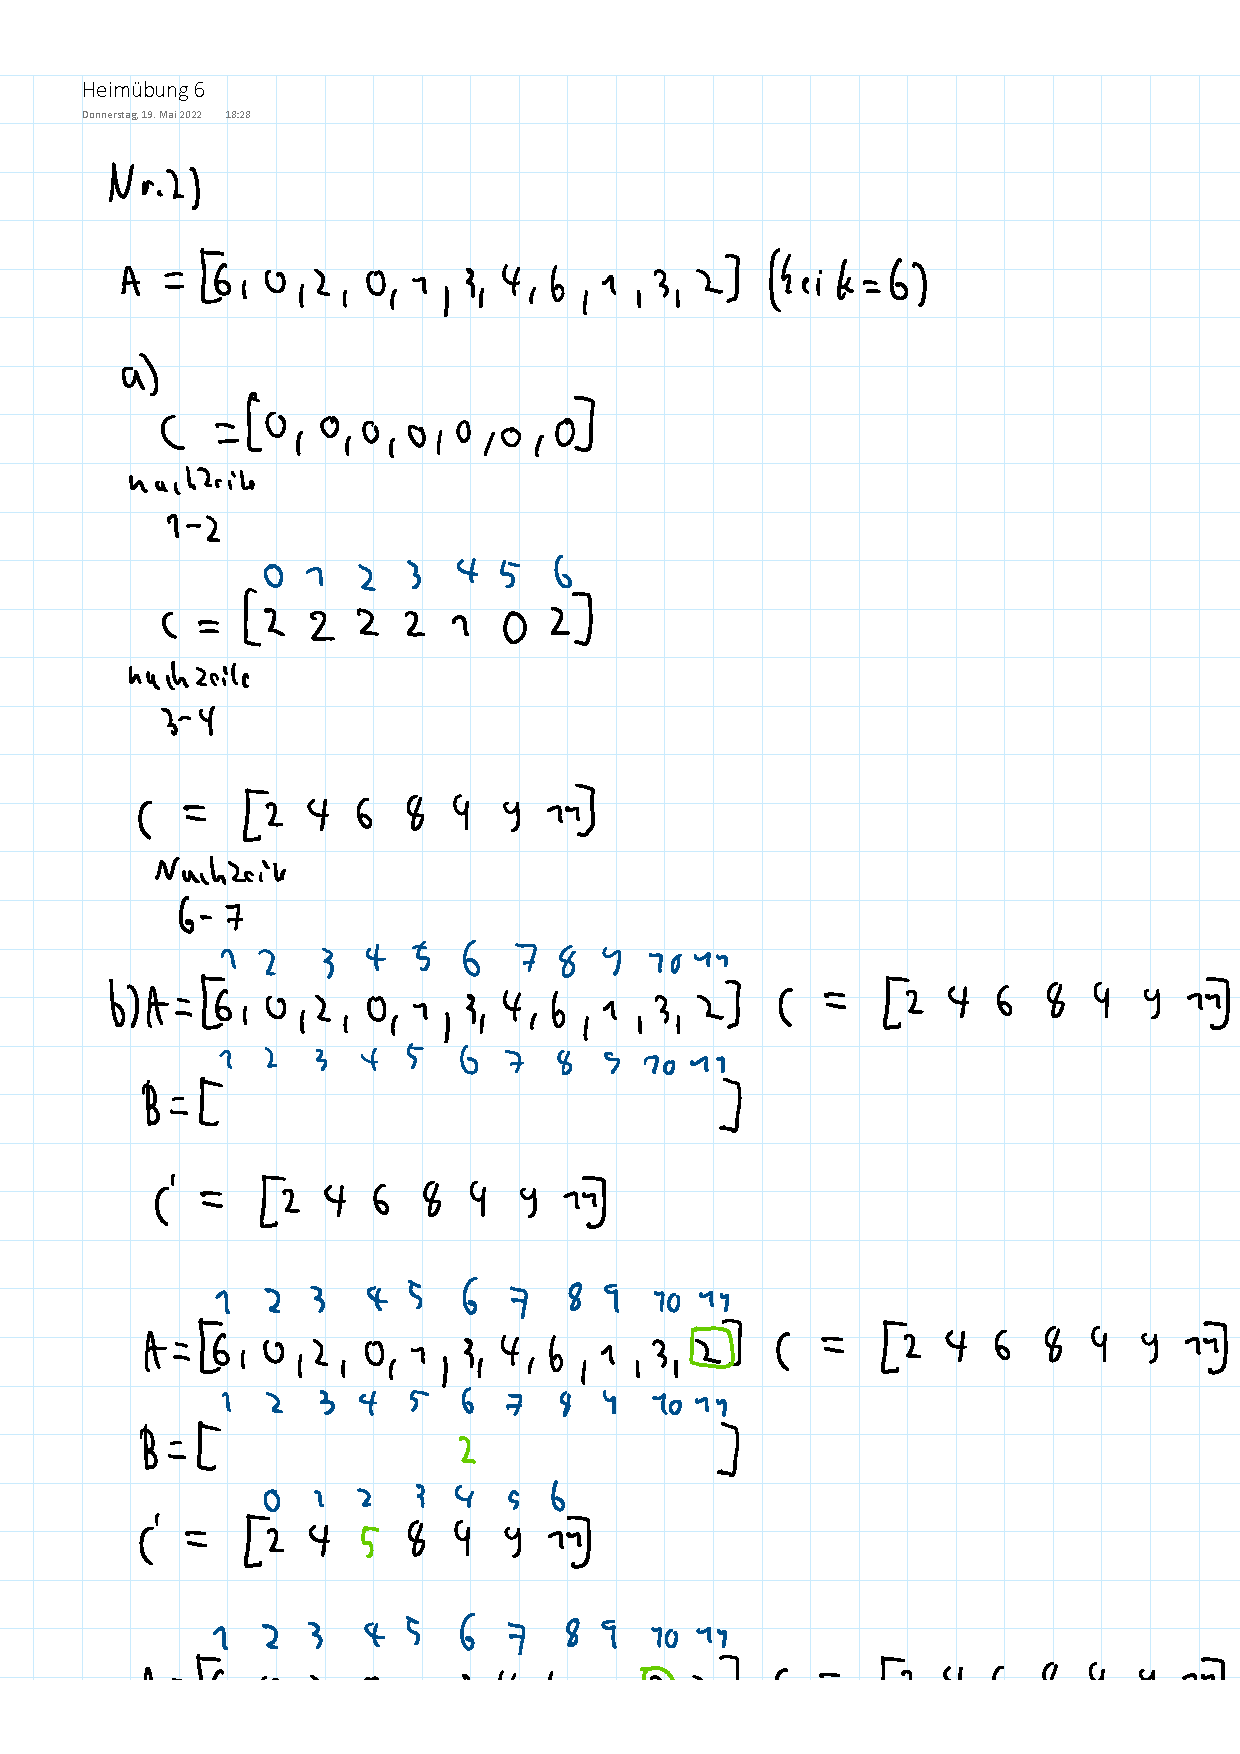
\includepdf[pages=-]{2022-05-19-Blatt-6-Aufgabe-2.pdf}

\end{aufgabe}

\begin{aufgabe}
  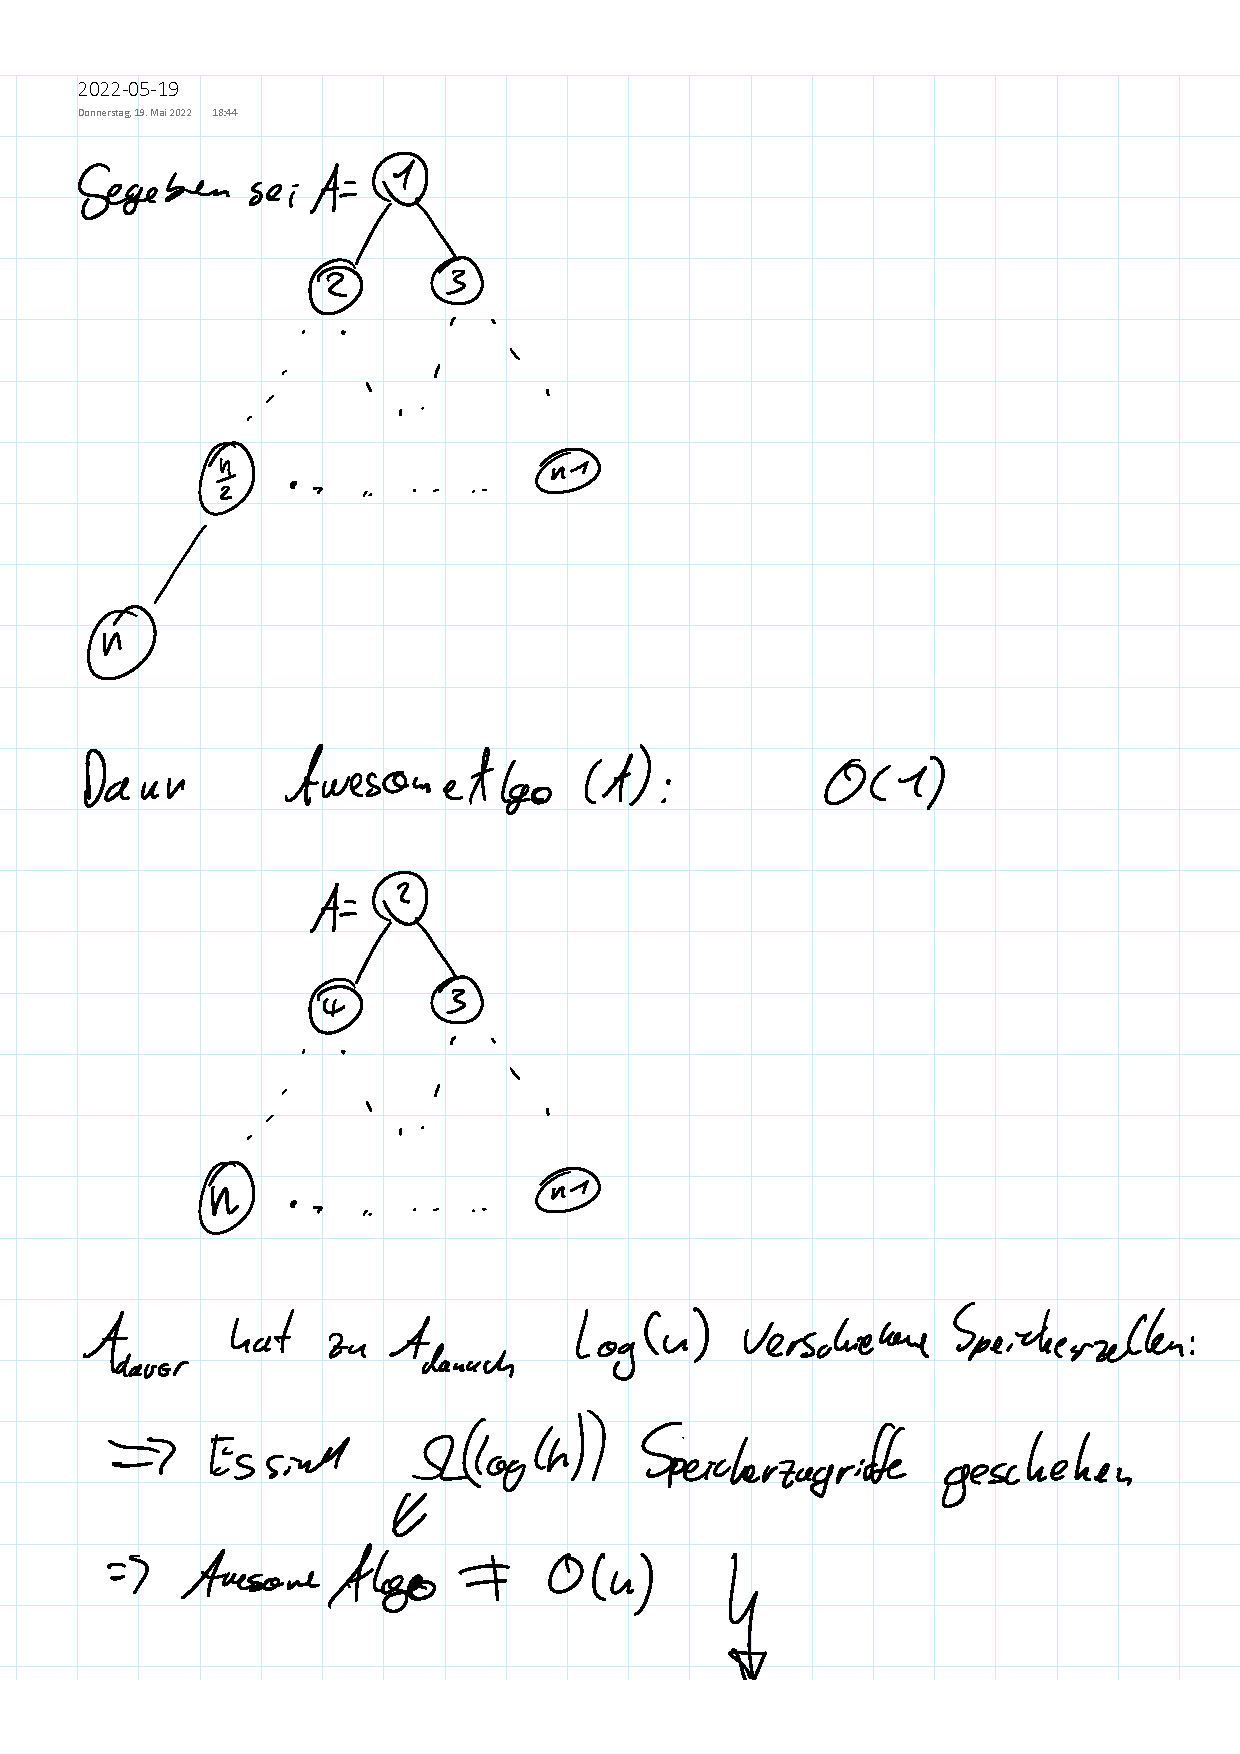
\includepdf[pages=-]{2022-05-19-Blatt-6-Aufgabe-3.pdf}
\end{aufgabe}
\end{document}
